CPU每取出并执行一条指令所需的全部时间,即CPU完成一条指令的时间,称为\textbf{指令周期}。

指令周期被划分为几个不同的阶段,\textbf{每个阶段所需的时间称为机器周期,}又称为CPU工作周期或基本周期,{\textbf{通常等于取指时间(或访存时间)。}}时钟周期是时钟频率的倒数,也可称为节拍脉冲或T周期,是处理操作最基本的单位。一个指令周期由若干个机器周期组成,每个机器周期又由若干个时钟周期组成,如下图所示。

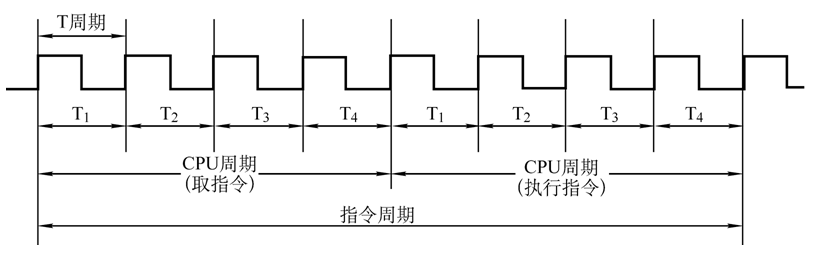
\includegraphics[width=3.46875in,height=1.07292in]{png-jpeg-pics/84CCBE908CB7911028A70F4E2C3D9F3F.png}

当CPU采用中断方式实现主存与I/O交换信息时,CPU在每条指令的执行周期结束前,都要发出\textbf{中断查询信号},以检测是否有I/O提出请求。如果有请求,则CPU要进入\textbf{中断响应阶段},又称为\textbf{中断周期}。这样,一个完整的指令周期应包括取指、间址、执行和中断4个子周期,如图5-7所示。{\textbf{完整的指令周期流程}}如图5-8所示。

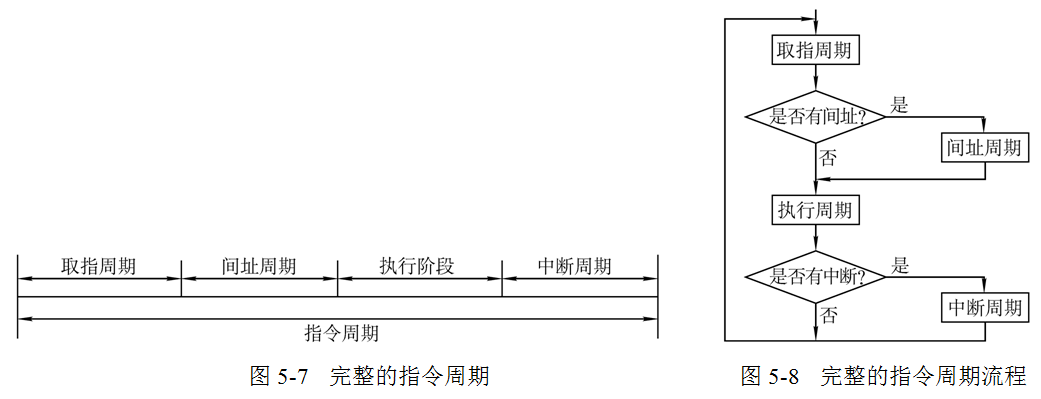
\includegraphics[width=3.59375in,height=1.37500in]{png-jpeg-pics/8086B5405CC83F4089C19FEBE6E5537B.png}
